%!TEX root = ../thesis.tex
\chapter{Results}
\label{ch:results}

\begin{itemize}
    \item Gleitenden Mittelwert bei Darstellung mit Window Size 20 um das Grundrauschen zu minimieren
    \item Konsistenz aller Modelle über die 5 Folds der Kreuzvalidierung ist gut, was eine robuste Trainierbarkeit bedeutet
\end{itemize}
\section{Oriented Bounding Boxes and Axis Aligned Bounding Boxes}
\begin{itemize}
    \item obb weil performance bei Map40-95 in allen Epochen besser
    \item Map bei obb zwiscehn 0.5 und 0.6; bei abb bei 0.35 und 0.45
    \item Bei gleichen Bounding box koordinaten ist obb bei 0.55 und 0.59 und abb 0.59 und 0.6
    \item bessere Performance von abb wahrscheinlich weil geringe Änderungen in der Orientierung der Bounding Boxen eine hohe Auswirkung auf die Genauigkeit der Boxen haben
\end{itemize}

\section{Comparision at Mean Average Precision 50-95}

\begin{figure}[h] 
    \centering % Centers the graphic horizontally
    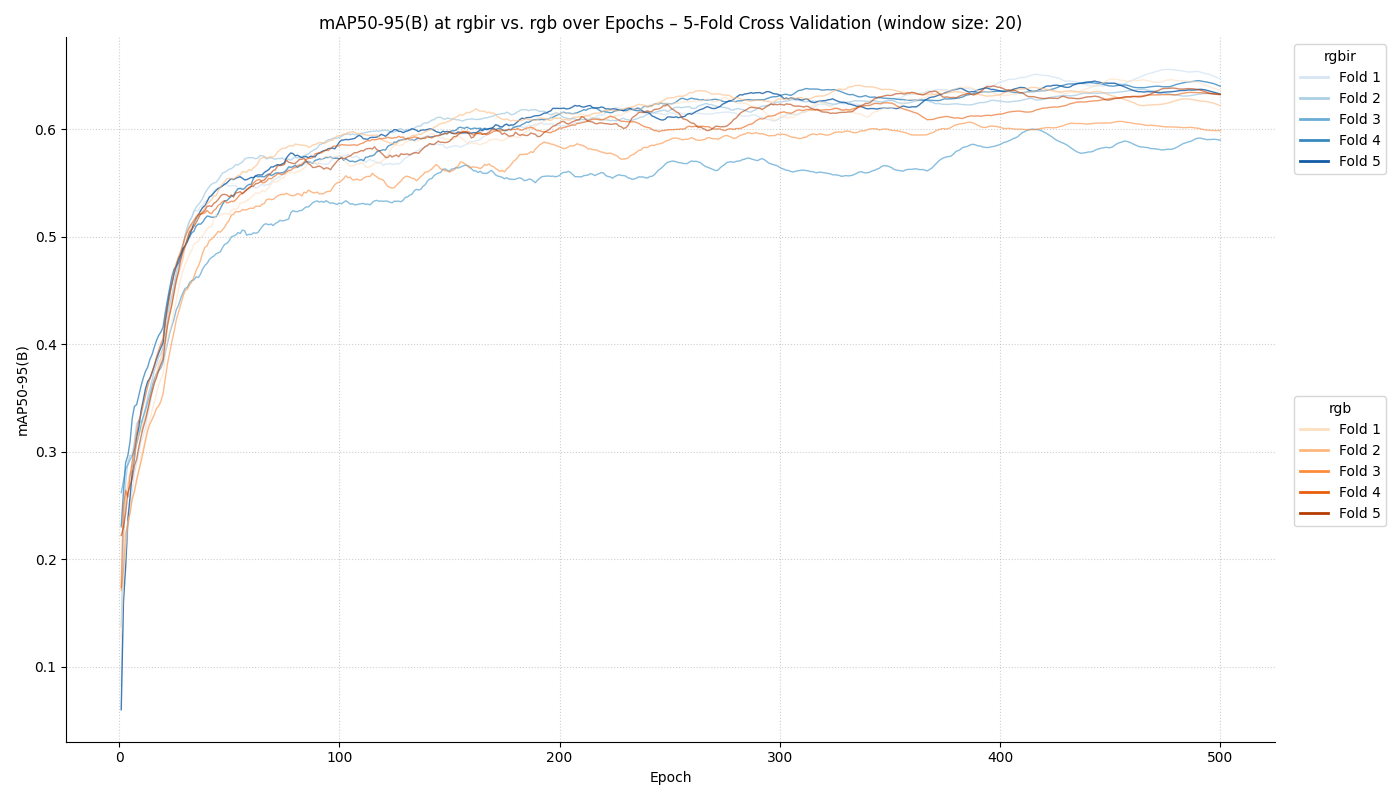
\includegraphics[width=1\textwidth]{images/rgbir/mAP@50-95/rgbir_vs_rgb_full.png} % Path to the graphic file
    \caption{Comparison of mAP50-95(B) over 500 Epochs for rgbir vs. rgb.} % Image caption
    \label{fig:map_rgbir_rgb} % Label for references in the text
\end{figure}
In Abb. \ref{fig:map_rgbir_rgb} ist ein Vergleich der mAP50-95 Werte für über die verschiedenen Eingabedatensätze RGBIR und RGB zu sehen. Hier wurde eine 5 Fold Cross Validation durchgeführt, um die Robustheit zu beurteilen. Insgesamt ist ein ansteigender Trend über alle Epochen hinweg zu beobachten. Der Anstieg der Leistung ist in den Anfangsepochen signifikanter und flacht dann ab, um im weiteren Verlauf bis Epoche 500 zu konvergieren. RGBIR hat bessere Spitzenleistung als RGB und erreicht konsequent höhere absolute mAP Werte. Über die längere Trainingsdauer verfestigt sich der anfängliche Vorteil von RGBIR. Die RGB-Modelle liegen bei einer mAP von 0.60-0.62, während die besten RGBIR Modelle Werte um 0.62-0.65 mAP erreichen. Die RGB-Modelle weisen eine höhere Streuung als die RGBIR-Modelle auf, die robsuter sind und konsistentere Resultate liefern. Ab Epoche 300-400 erreichen beide Modelle ein Plateu, ab dem die Leistung nur noch geringfügig schwankt, was darauf hindeutet, dass die Modelle weitgehend konvergiert sind.

\begin{figure}[h] 
    \centering % Centers the graphic horizontally
    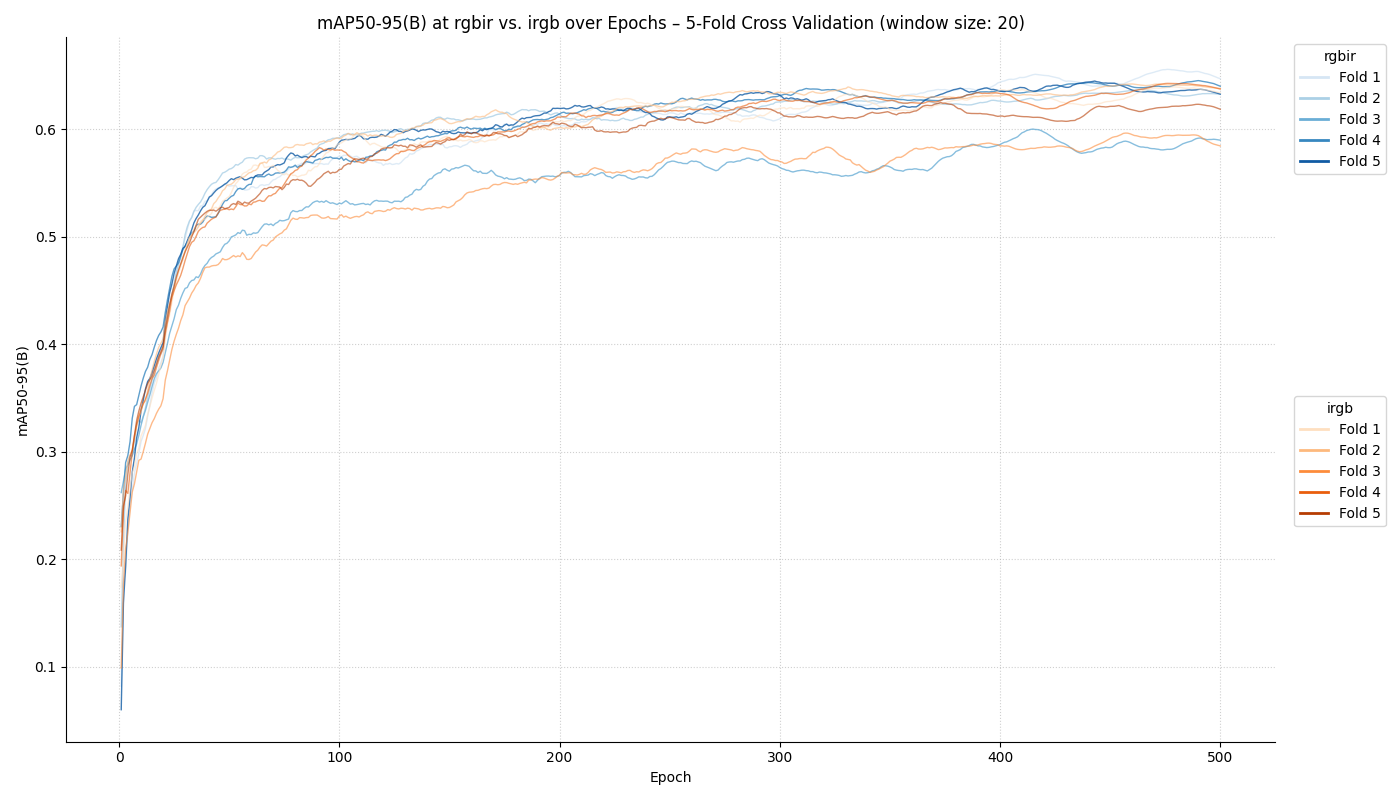
\includegraphics[width=1\textwidth]{images/rgbir/mAP@50-95/rgbir_vs_irgb_full.png} % Path to the graphic file
    \caption{Comparison of mAP50-95(B) over 500 Epochs for rgbir vs. irgb.} % Image caption
    \label{fig:map_rgbir_irgb} % Label for references in the text
\end{figure}
Aus Abb.\ref{fig:map_rgbir_irgb}, welche einen Vergleich der RGBIR- und IRGB-Modelle zeigt, ist ebenfalls ein klarer Performance Vorteil von RGBIR ersichtlich. Die IRGB-Modelle lernen zwar ebenfalls schnell, haben aber stärkere Schwankungen in den einzelnen Folds. Das Plateau der IRGB-Modelle liegt niedriger als bei RGBIR zwischen ca. 0.56 und 0.60. Es ist auffällig, dass die Konvergenz teilweise instabil ist, da manche Folds niedrigere Werte aufweisen. Außerdem erreicht keine einzige Fold Linie der IRGB-Modelle das Niveau der RGBIR-Modelle. \todo{Text an andere Beschreibungen anpassen (immer gleiches Schema verwenden?)}

\begin{figure}[h] 
    \centering % Centers the graphic horizontally
    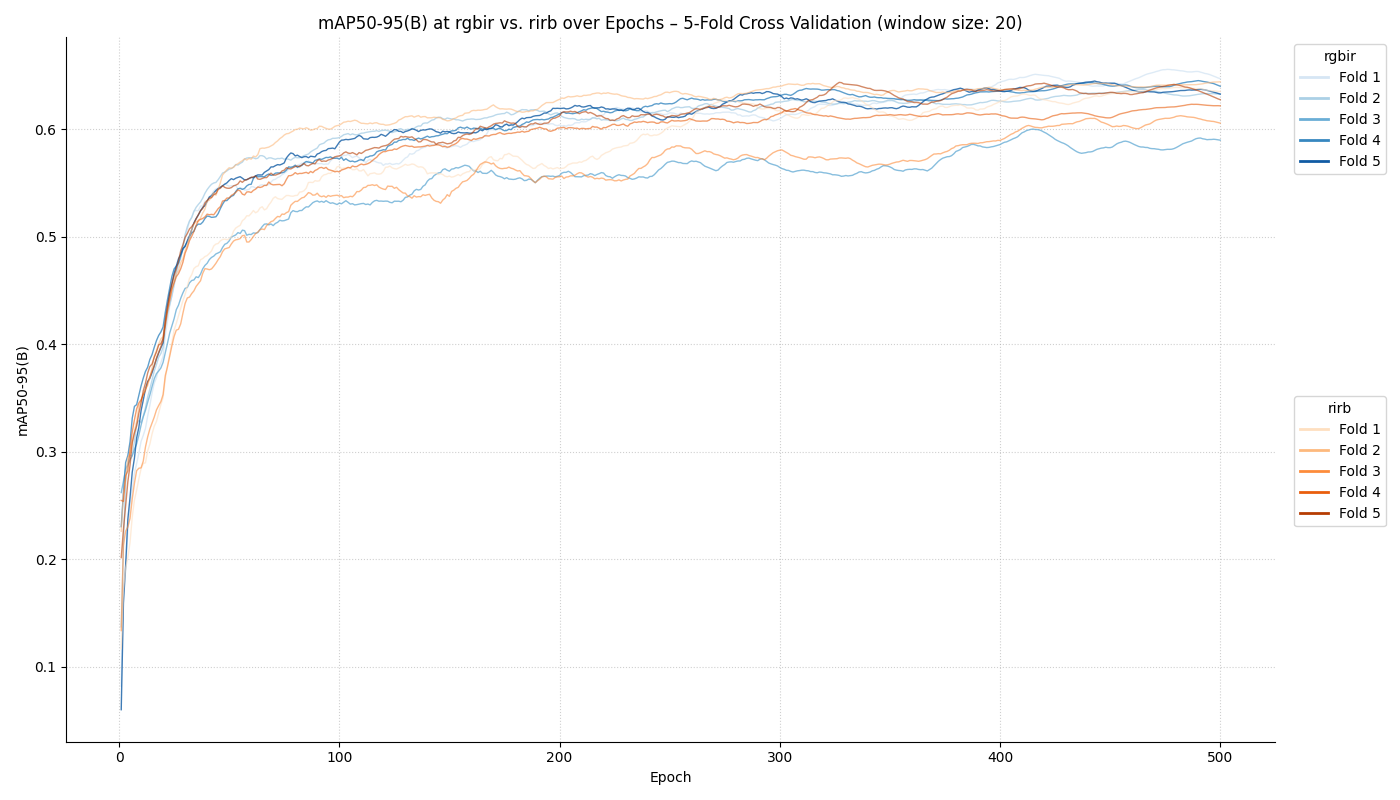
\includegraphics[width=1\textwidth]{images/rgbir/mAP@50-95/rgbir_vs_rirb_full.png} % Path to the graphic file
    \caption{Comparison of mAP50-95(B) over 500 Epochs for rgbir vs. rirb.} % Image caption
    \label{fig:map_rgbir_rirb} % Label for references in the text
\end{figure}
Die Abb. \ref{fig:map_rgbir_rirb} veranschaulicht die Leistungsentwicklung zwischen dem RGBIR- und RIRB-Modellen. Zunächst steigt der mAP Wert aller Folds sehr stark an, wie es in den ersten 150 Epochen zu sehen ist. Auch beim RIRB-Modell verlangsamt sich der Anstieg im weiteren Verlauf deutlich, bis die Kurven gegen Ende der Trainingszeit ein Plateau erreichen. Bis zu den 500 Epochen haben die meisten Folds ihren Höhepunkt erreicht oder sich diesem angenähert. \\
Zu Beginn des Trainings in den ersten 150 Epochen ist die Leistung beider Modelle sehr ähnlich. Die orangen und blauen Kurven verlaufen in dieser Phase meist sehr eng beieinander und überschneiden sich häufig. In der mittleren bis späteren Phase (150 bis 500 Epochen) ist wieder zu sehen, dass das RGBIR-Modell sich von seinem Pendant absetzt, da die mAP Werte oberhalb der von dem RIRB-Modell liegen, was auf eine bessere Objekterkennung hindeutet. Hier ist insbesondere der Fold 3 des RGBIR-Modelles auffällig, da er die höchsten mAP Werte über viele der späteren Epochen erreicht, die häufig Werte über 0.6 erreichen und gelegentlich sogar nahe an 0.65 heranreichen. Es ist jedoch zu bemerken, dass einige Folds der RIRB-Modelle (z. B. Fold 4) ebenfalls gute mAP Werte erreichen und sich manchen RGBIR Folds annäheren oder diese übertreffen. Insgesamt ist jedoch die durchschnittliche Leistung von RGBIR besser. \\
Die Leistung des RGBIR-Modelles ist über die 5 Folds relativ konsistent, da alle Folds ähnliche Trends aufweisen. Fold 3 weicht leicht positiv vom Rest ab, da er besonders hohe Genauigkeitswerte erzielt. Bei dem RIRB-Modell ist die Leistung über die Folds ebenfalls konsistent. Die Streuung zwischen den Folds ist vergleichbar mit dem RGBIR-Modell. Hier zeigt kein Fold ein drastisch schlechteres Verhalten als die anderen. \\

\begin{figure}[h] 
    \centering % Centers the graphic horizontally
    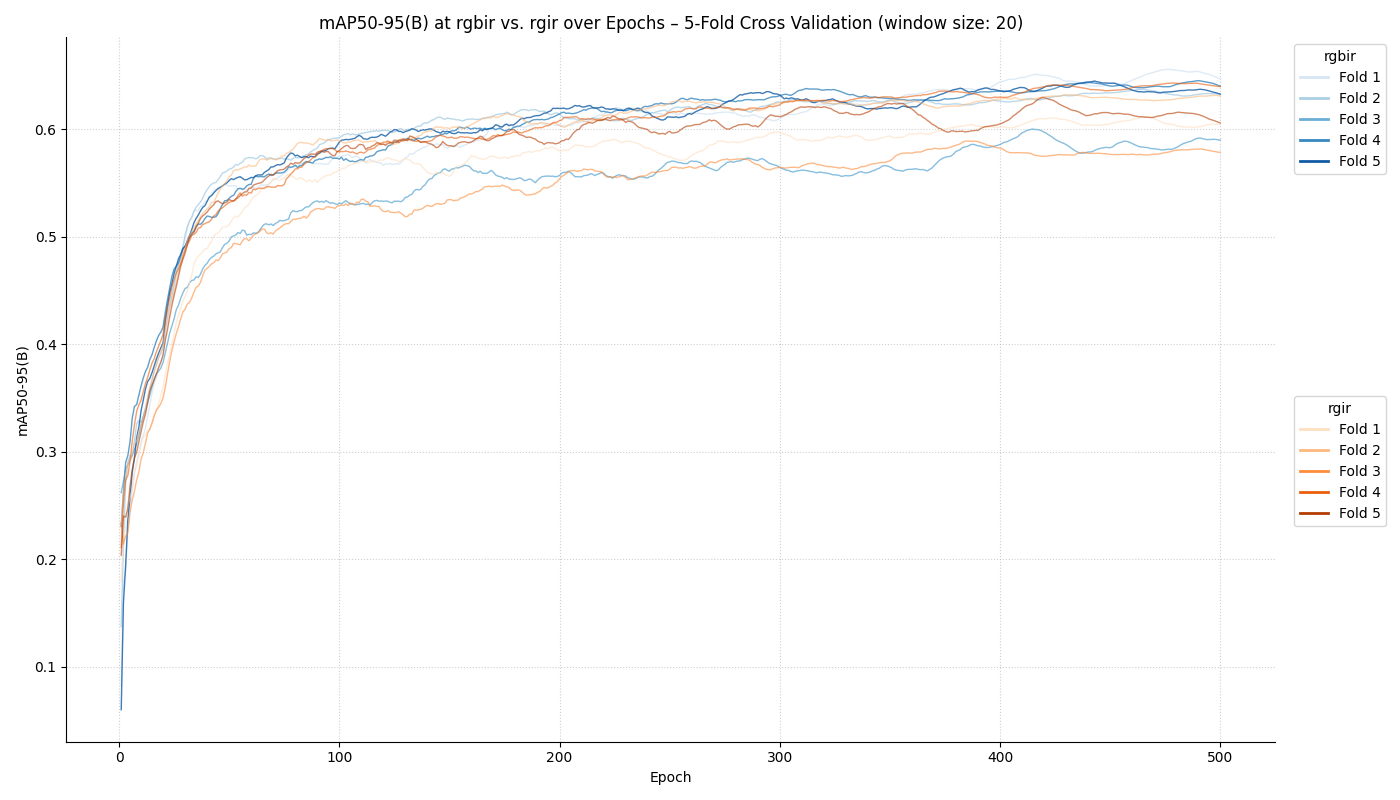
\includegraphics[width=1\textwidth]{images/rgbir/mAP@50-95/rgbir_vs_rgir_full.png} % Path to the graphic file
    \caption{Comparison of mAP50-95(B) over 500 Epochs for rgbir vs. rgir.} % Image caption
    \label{fig:map_rgbir_rgir} % Label for references in the text
\end{figure}
Zu Beginn zeigen beide Modelle bei Vergleich von dem RGBIR- und RGIR-Modell in Abb. \ref{fig:map_rgbir_rgir} einen typischen Verlauf mit steilem Anstieg, gefolgt von einer Verlangsamung und schließlich einer Stabilisierung der Leistung. Während der ersten 150 Epochen verlaufen die Kurven beider Modelle nahezu identisch, ohne dass sich eines deutlich absetzt. Es ist kein Leistungsvorsprung für eines der beiden Modelle zu sehen. In den mittleren bis späteren Epochen ist im Gegensatz zu den RGB-, IRGB- und RIRB-Modellen eine sehr ähnliche oder tendenziell bessere Performance abgebildet. Besonders Fold 4 und Fold 5 des RGIR-Modells fallen durch stabile und hohe mAP-Werte auf, die mit den besten Ergebnissen des RGBIR-Modells mithalten können oder sie stellenweise übertreffen. In den späteren Trainingsphasen zeigen die RGIR-Folds eine größere Varianz nach oben, was darauf hinweist, dass einzelne Folds besonders hohe Genauigkeitswerte erreichen können. \\
Das RGIR-Modell ist eine gute Alternative zum RGBIR-Modell, da es eine potenziell überlegene Leistung bietet. Diese ist in den späteren Trainingsphasen zu erkennen, wo das RGIR-Modell ein gleichwertiges oder besseres Ergebnis erzielt. Dadurch ist es möglich, dass das RGIR-Modell eine ähnlich starke oder in einzelnen Fällen sogar überlegene Leistung zeigen könnte wie das RGBIR-Modell.



\begin{figure}[h] 
    \centering % Centers the graphic horizontally
    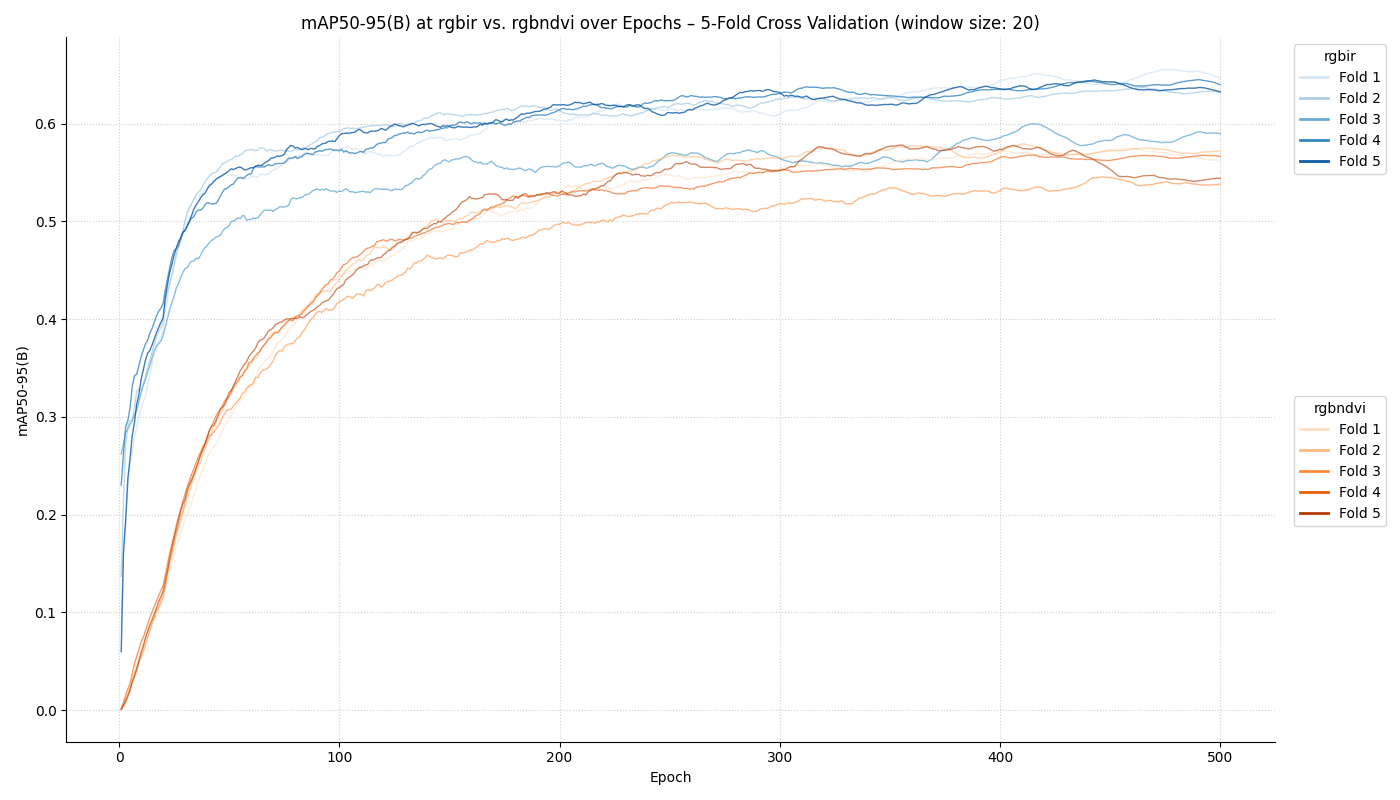
\includegraphics[width=1\textwidth]{images/rgbir/mAP@50-95/rgbir_vs_rgbndvi_full.png} % Path to the graphic file
    \caption{Comparison of mAP50-95(B) over 500 Epochs for rgbir vs. rgbndvi.} % Image caption
    \label{fig:map_rgbir_rgbndvi} % Label for references in the text
\end{figure}

\begin{figure}[h] 
    \centering % Centers the graphic horizontally
    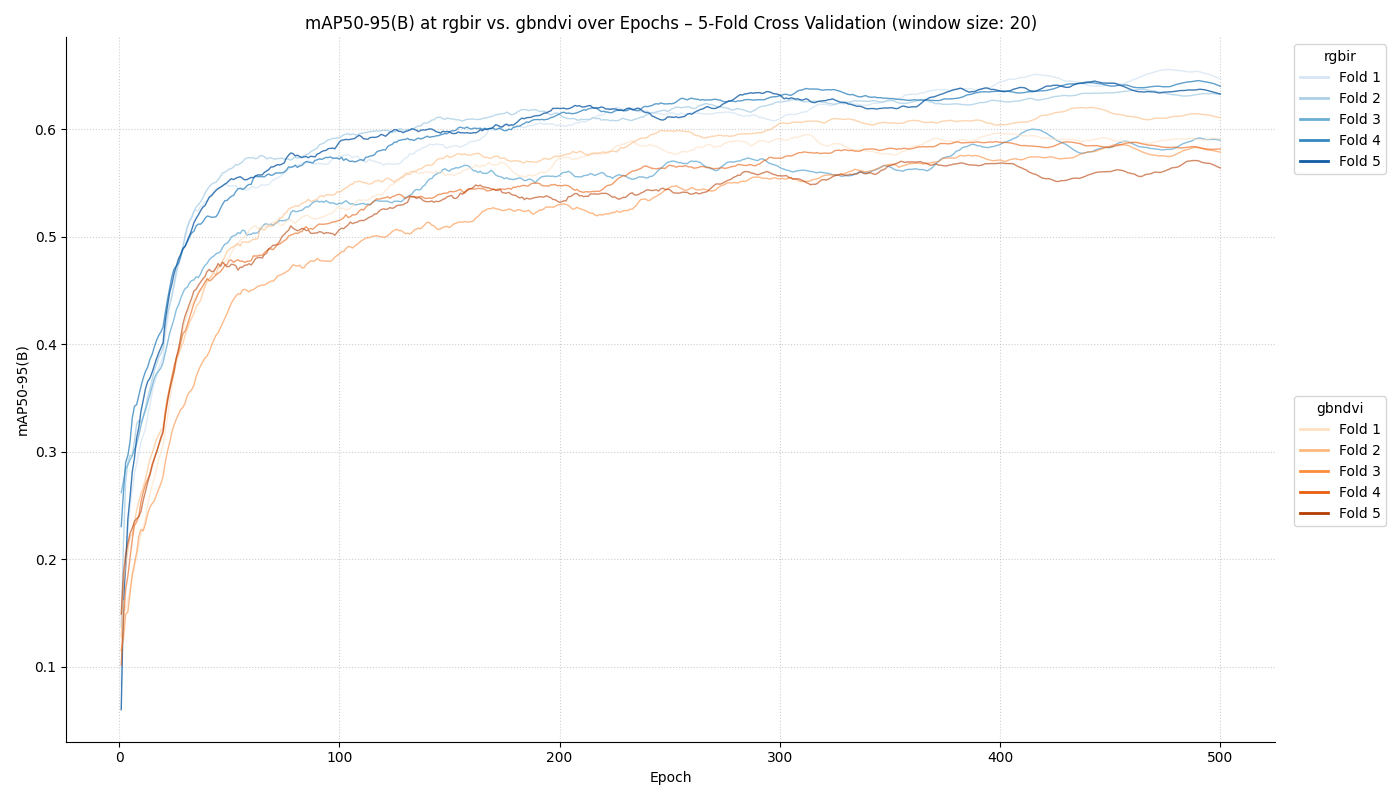
\includegraphics[width=1\textwidth]{images/rgbir/mAP@50-95/rgbir_vs_gbndvi_full.png} % Path to the graphic file
    \caption{Comparison of mAP50-95(B) over 500 Epochs for rgbir vs. gbndvi.} % Image caption
    \label{fig:map_rgbir_gbndvi} % Label for references in the text
\end{figure}

Als weitere Variante wurde der NDVI-Index als zusätzlicher Kanal zu den RGB-Daten (RGBNDVI-Modell) sowie einmal nur zu den Grün- und Blau-Kanälen (GBNDVI-Modell) hinzugefügt. Aufgrund der ähnlichen Ergebnisse werden die Resultate beider Modelle, die in den Abb. \ref{fig:map_rgbir_rgbndvi} (RGBNDVI) und \ref{fig:map_rgbir_gbndvi} (GBNDVI) mit dem RGBIR Modell zu sehen sind, im Folgenden gemeinsam verglichen. In beiden Abbildungen zeigt sich in den ersten 150 Epochen ein deutlicher Vorsprung des RGBIR-Modells: Die Kurven steigen schneller an und erreichen früh höhere mAP-Werte. Das RGBNDVI-Modell und auch das GBNDVI-Modell holen deutlich langsamer auf. In der mittleren Phase (150–500 Epochen) vergrößert sich der Leistungsunterschied weiter. Das RGBIR-Modell zeigt durchweg eine deutlich bessere Performance im Vergleich zu den RGBNDVI- und GBNDVI-Modellen. 


\section{Comparision with Confusion Matrices}
\begin{figure}[h] 
    \centering
    % Erste Subfigur
    \begin{subfigure}[b]{0.85\textwidth} % [b] für bottom alignment, 0.48\textwidth damit noch Platz ist
        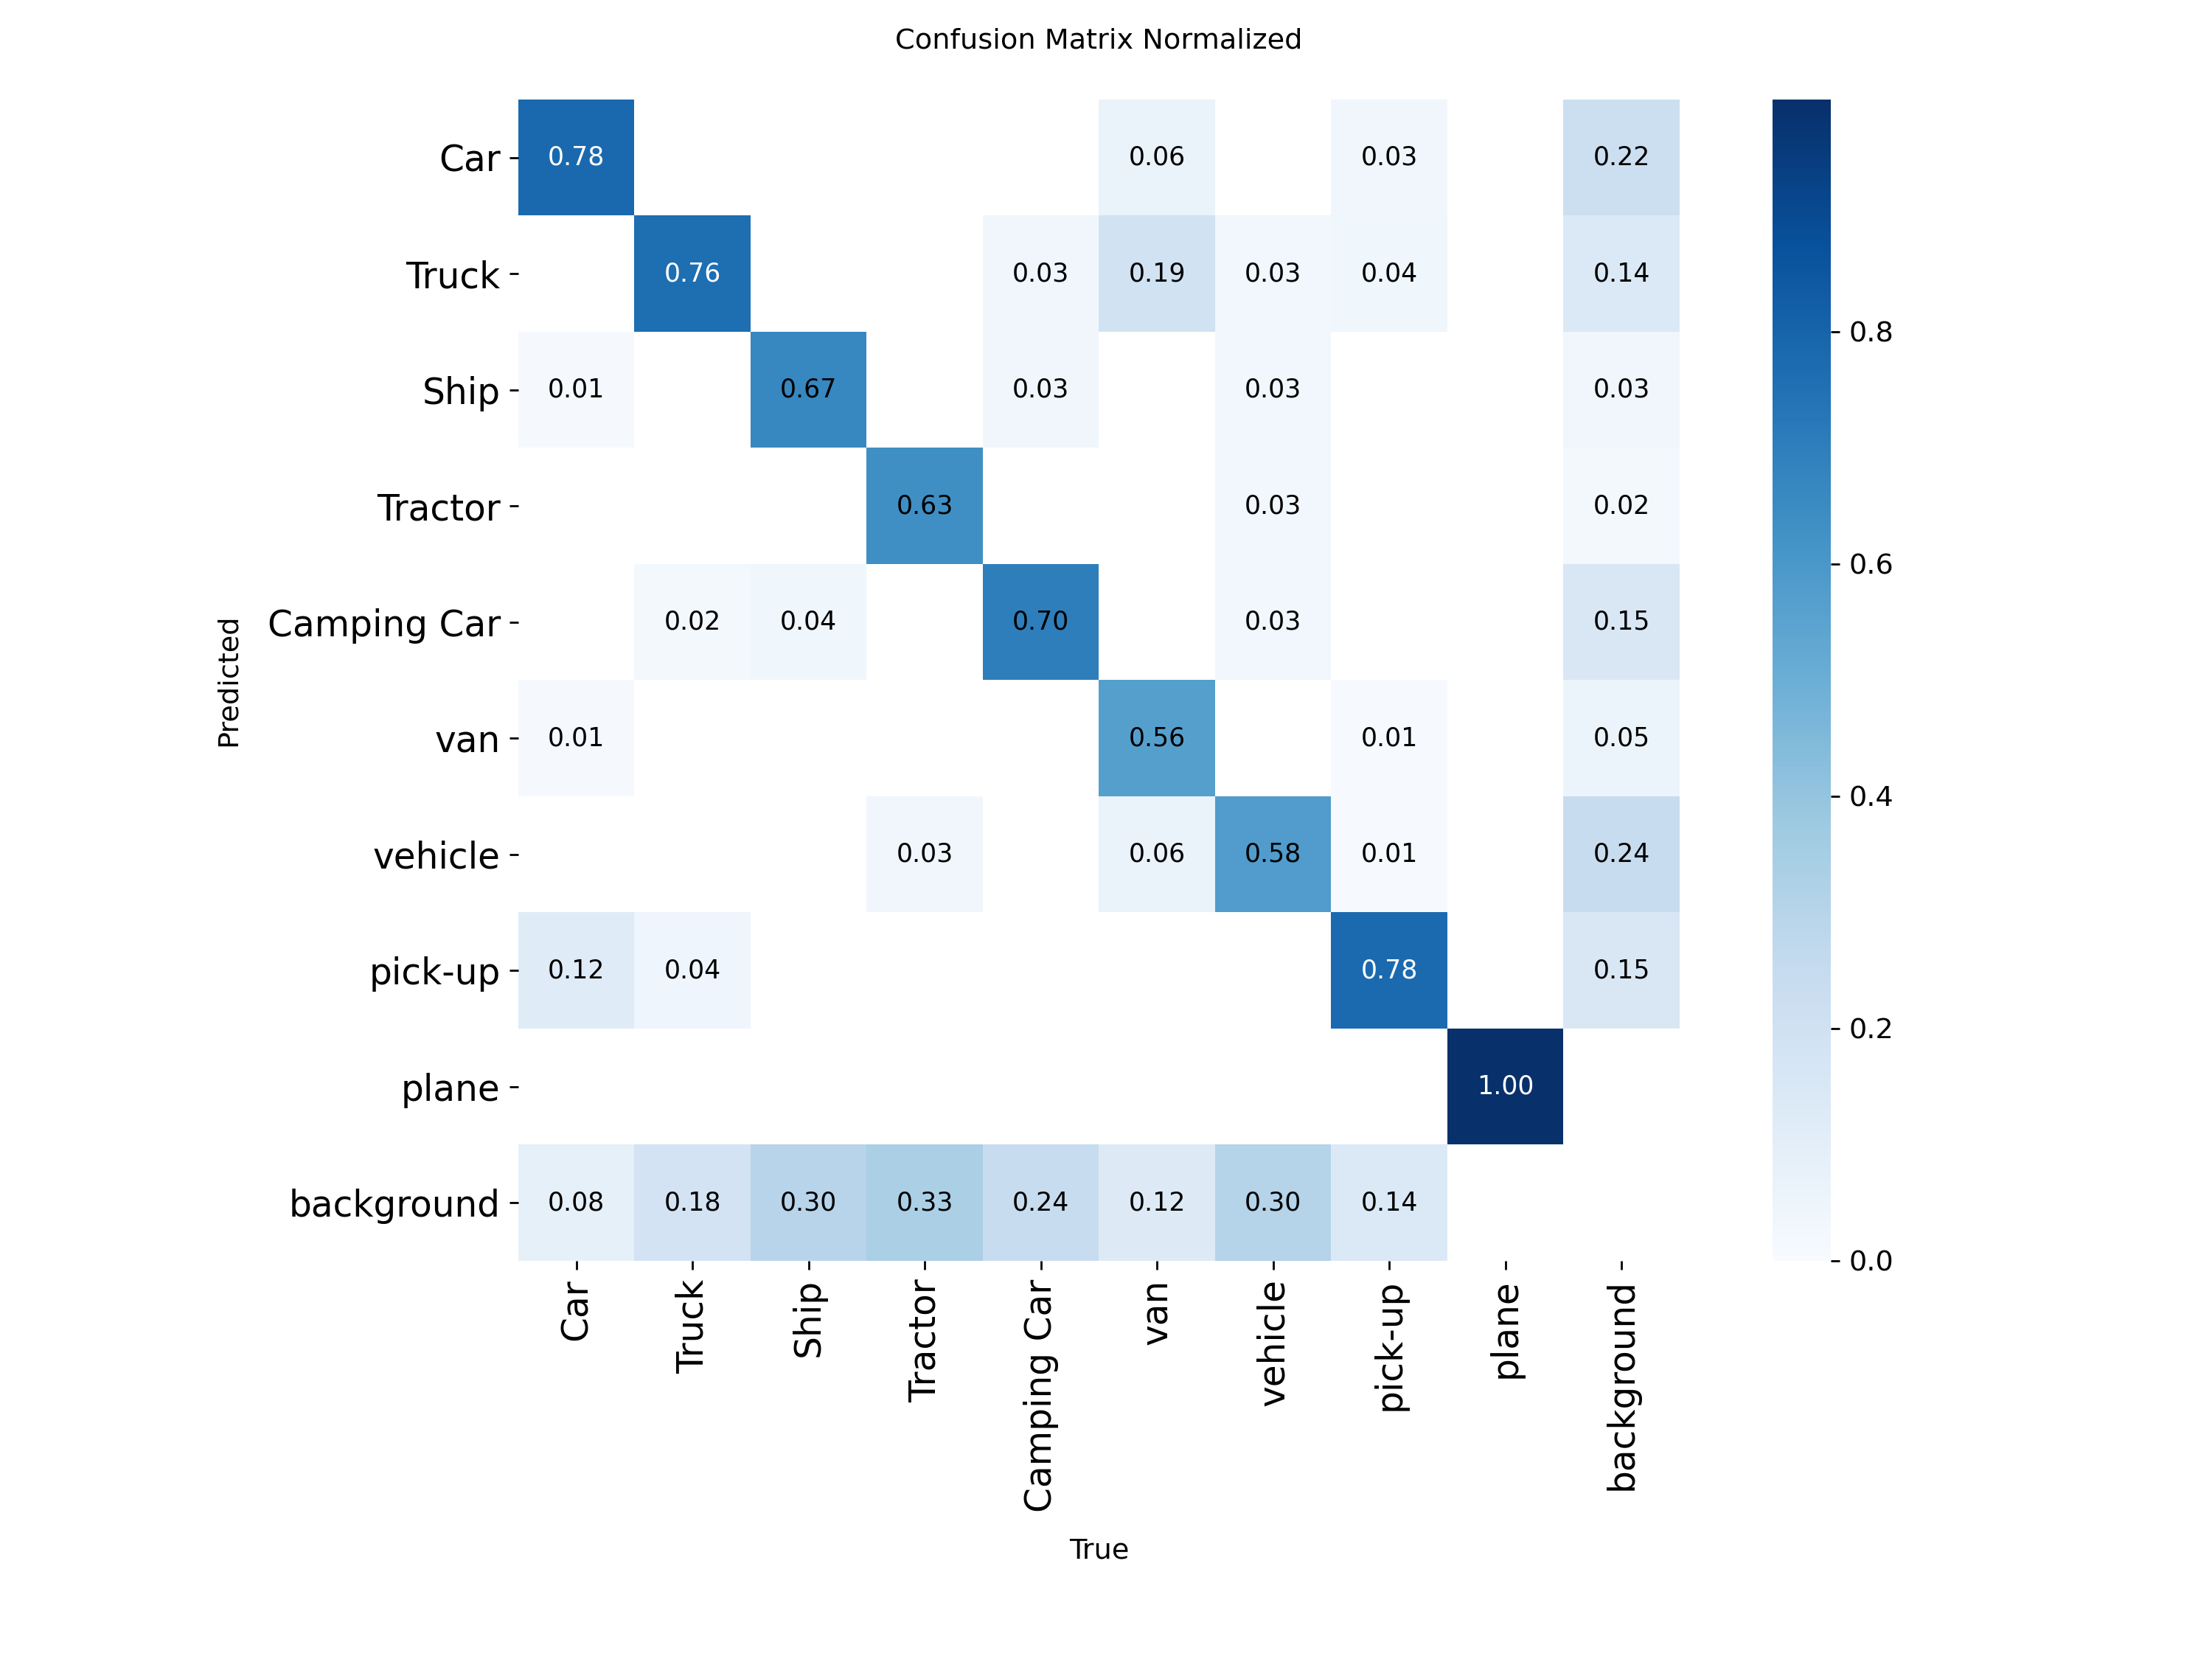
\includegraphics[width=\textwidth]{images/confusion_matrices/rgbir_F4_confusion_matrix_normalized.png} % Bildpfad zum ersten Bild
        \caption{r-g-b-ir} % Unterschrift für das erste Bild
        \label{fig:cm_rgbir} % Label für Referenzierung von Bild 1
    \end{subfigure}
    \hfill % Fügt horizontalen Platz zwischen den Subfiguren ein
    % Zweite Subfigur
    \begin{subfigure}[b]{0.85\textwidth} % 0.48\textwidth für das zweite Bild
        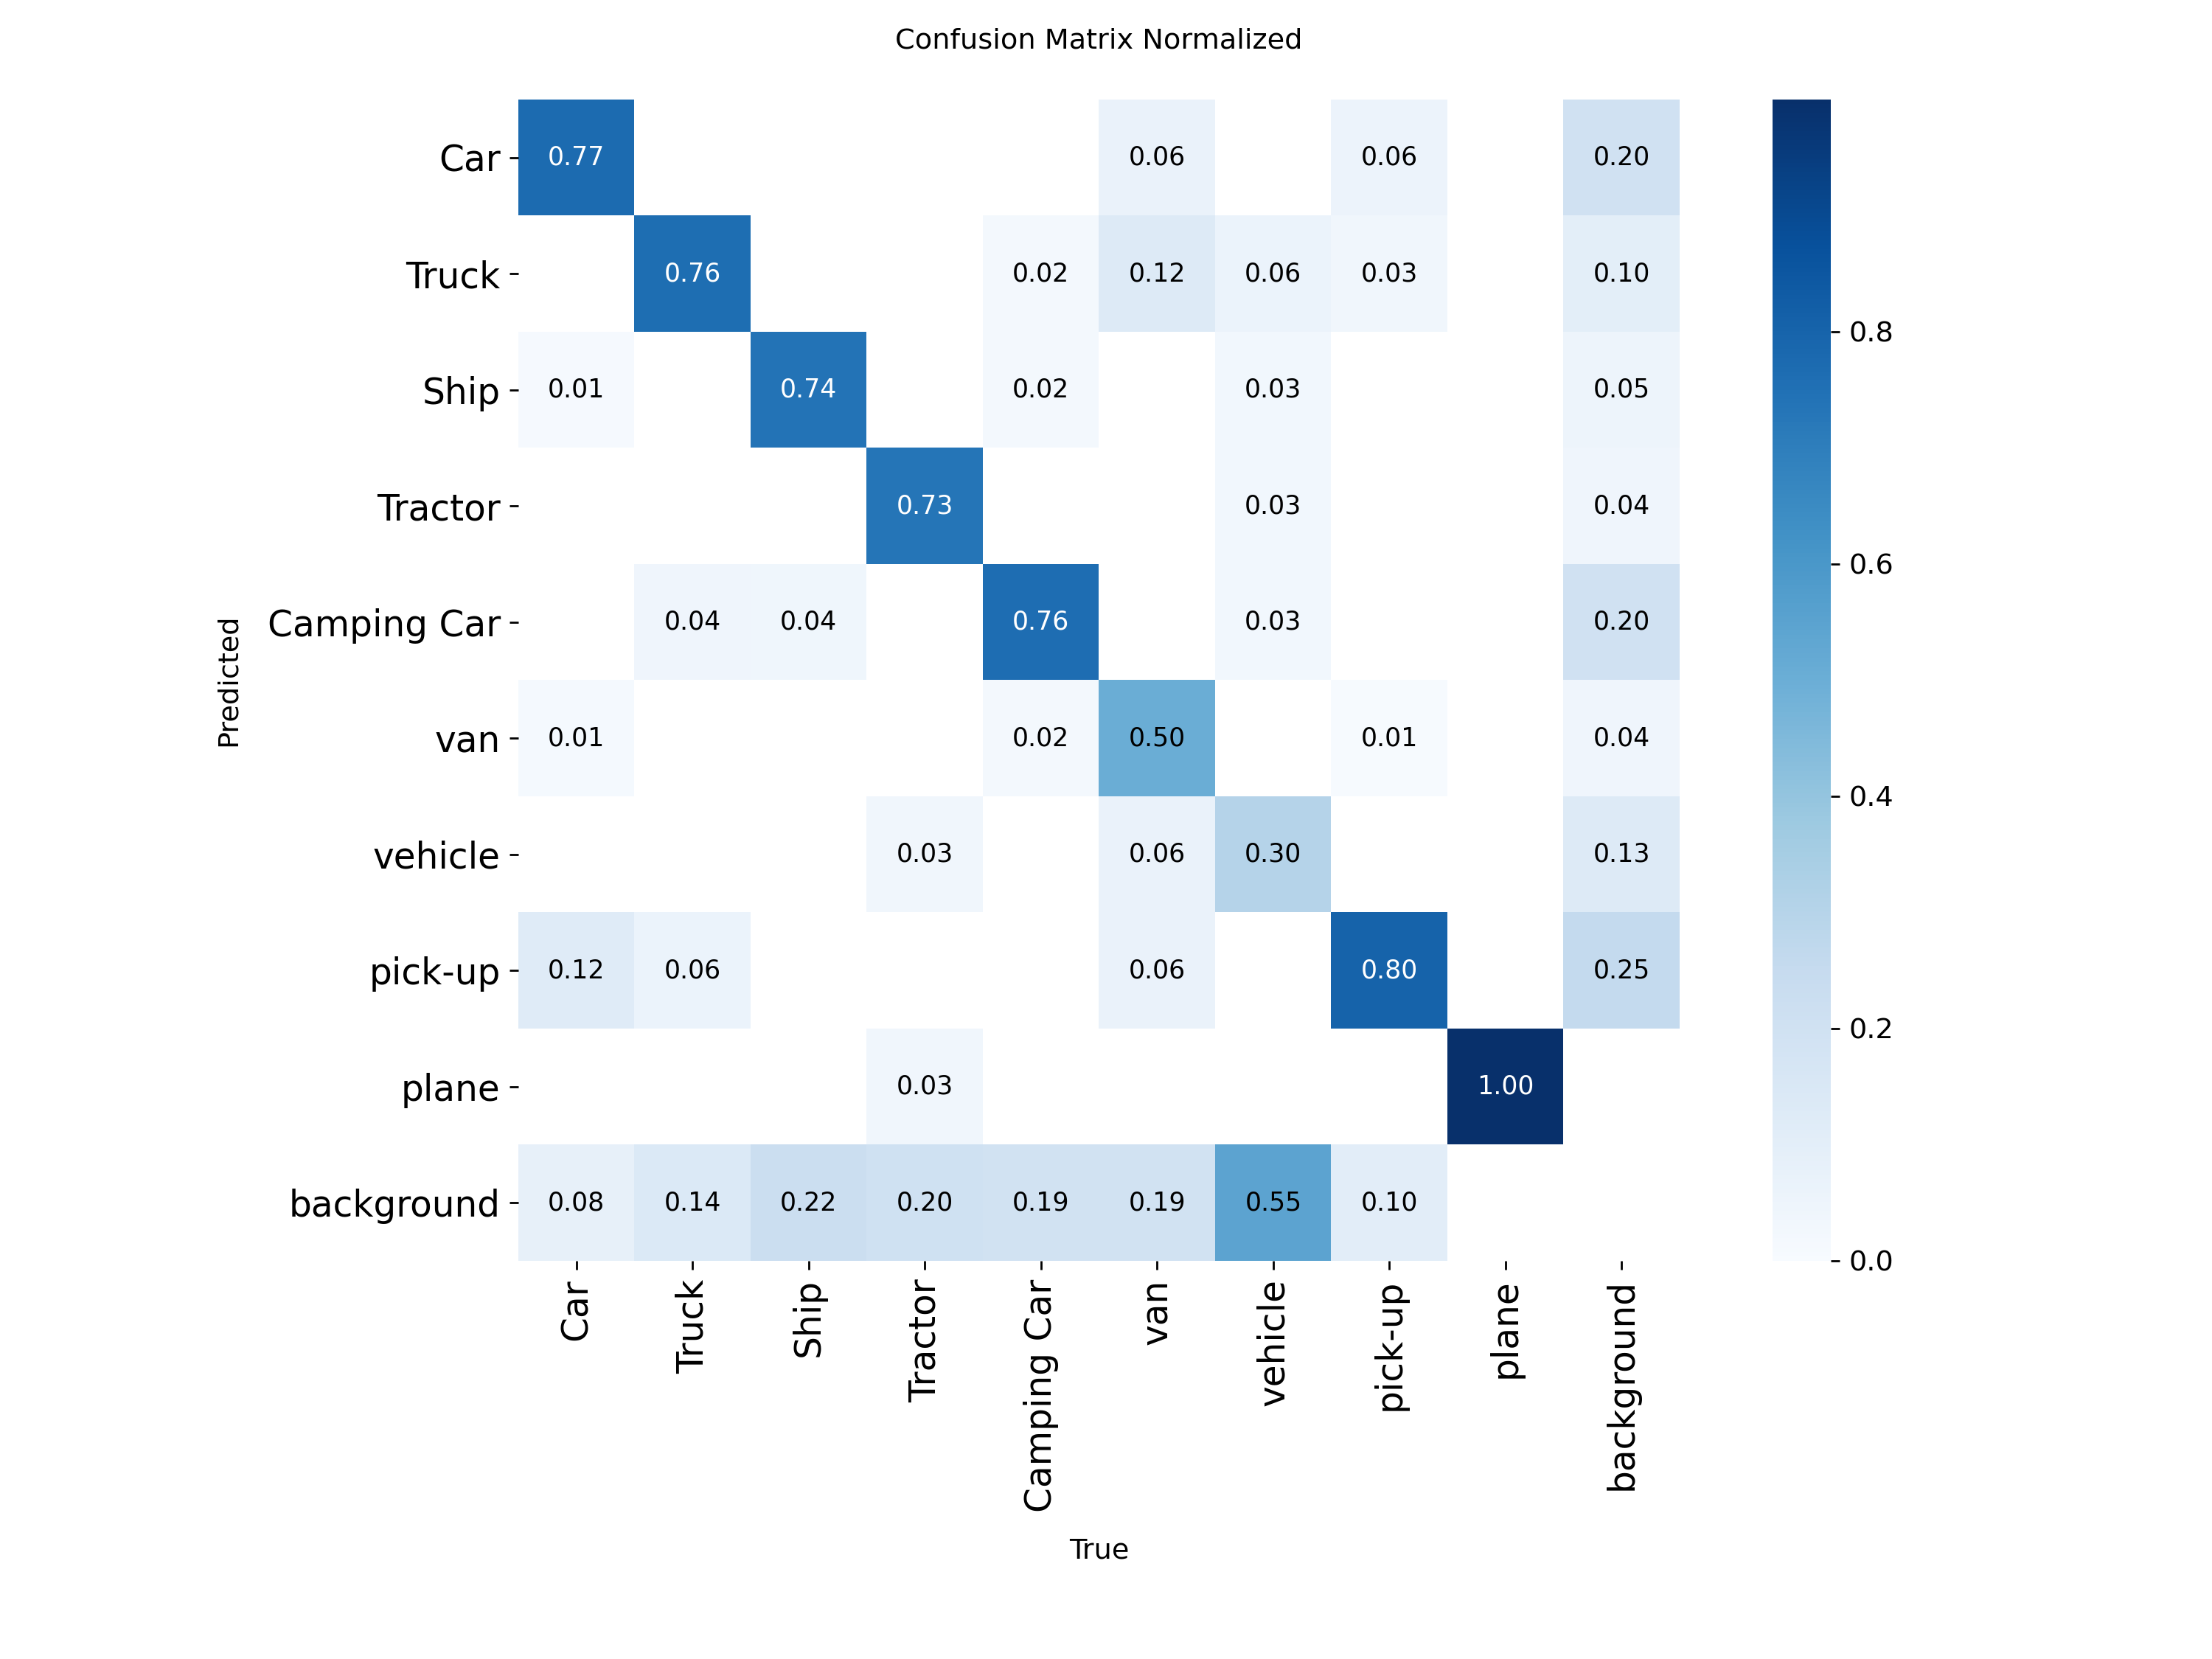
\includegraphics[width=\textwidth]{images/confusion_matrices/irgb_F4_confusion_matrix_normalized.png} % Bildpfad zum zweiten Bild
        \caption{ir-g-b} % Unterschrift für das zweite Bild
        \label{fig:cm_irgb} % Label für Referenzierung von Bild 2
    \end{subfigure}
    \caption{Comparison of Confusion Matrices between r-g-b-ir und ir-g-b for Fold 4} % Gemeinsame Unterschrift für beide Bilder
    \label{fig:combined_maps} % Label für die gesamte Figure-Umgebung
\end{figure}

\begin{figure}[h] 
    \centering
    % Erste Subfigur
    \begin{subfigure}[b]{0.85\textwidth} % [b] für bottom alignment, 0.48\textwidth damit noch Platz ist
        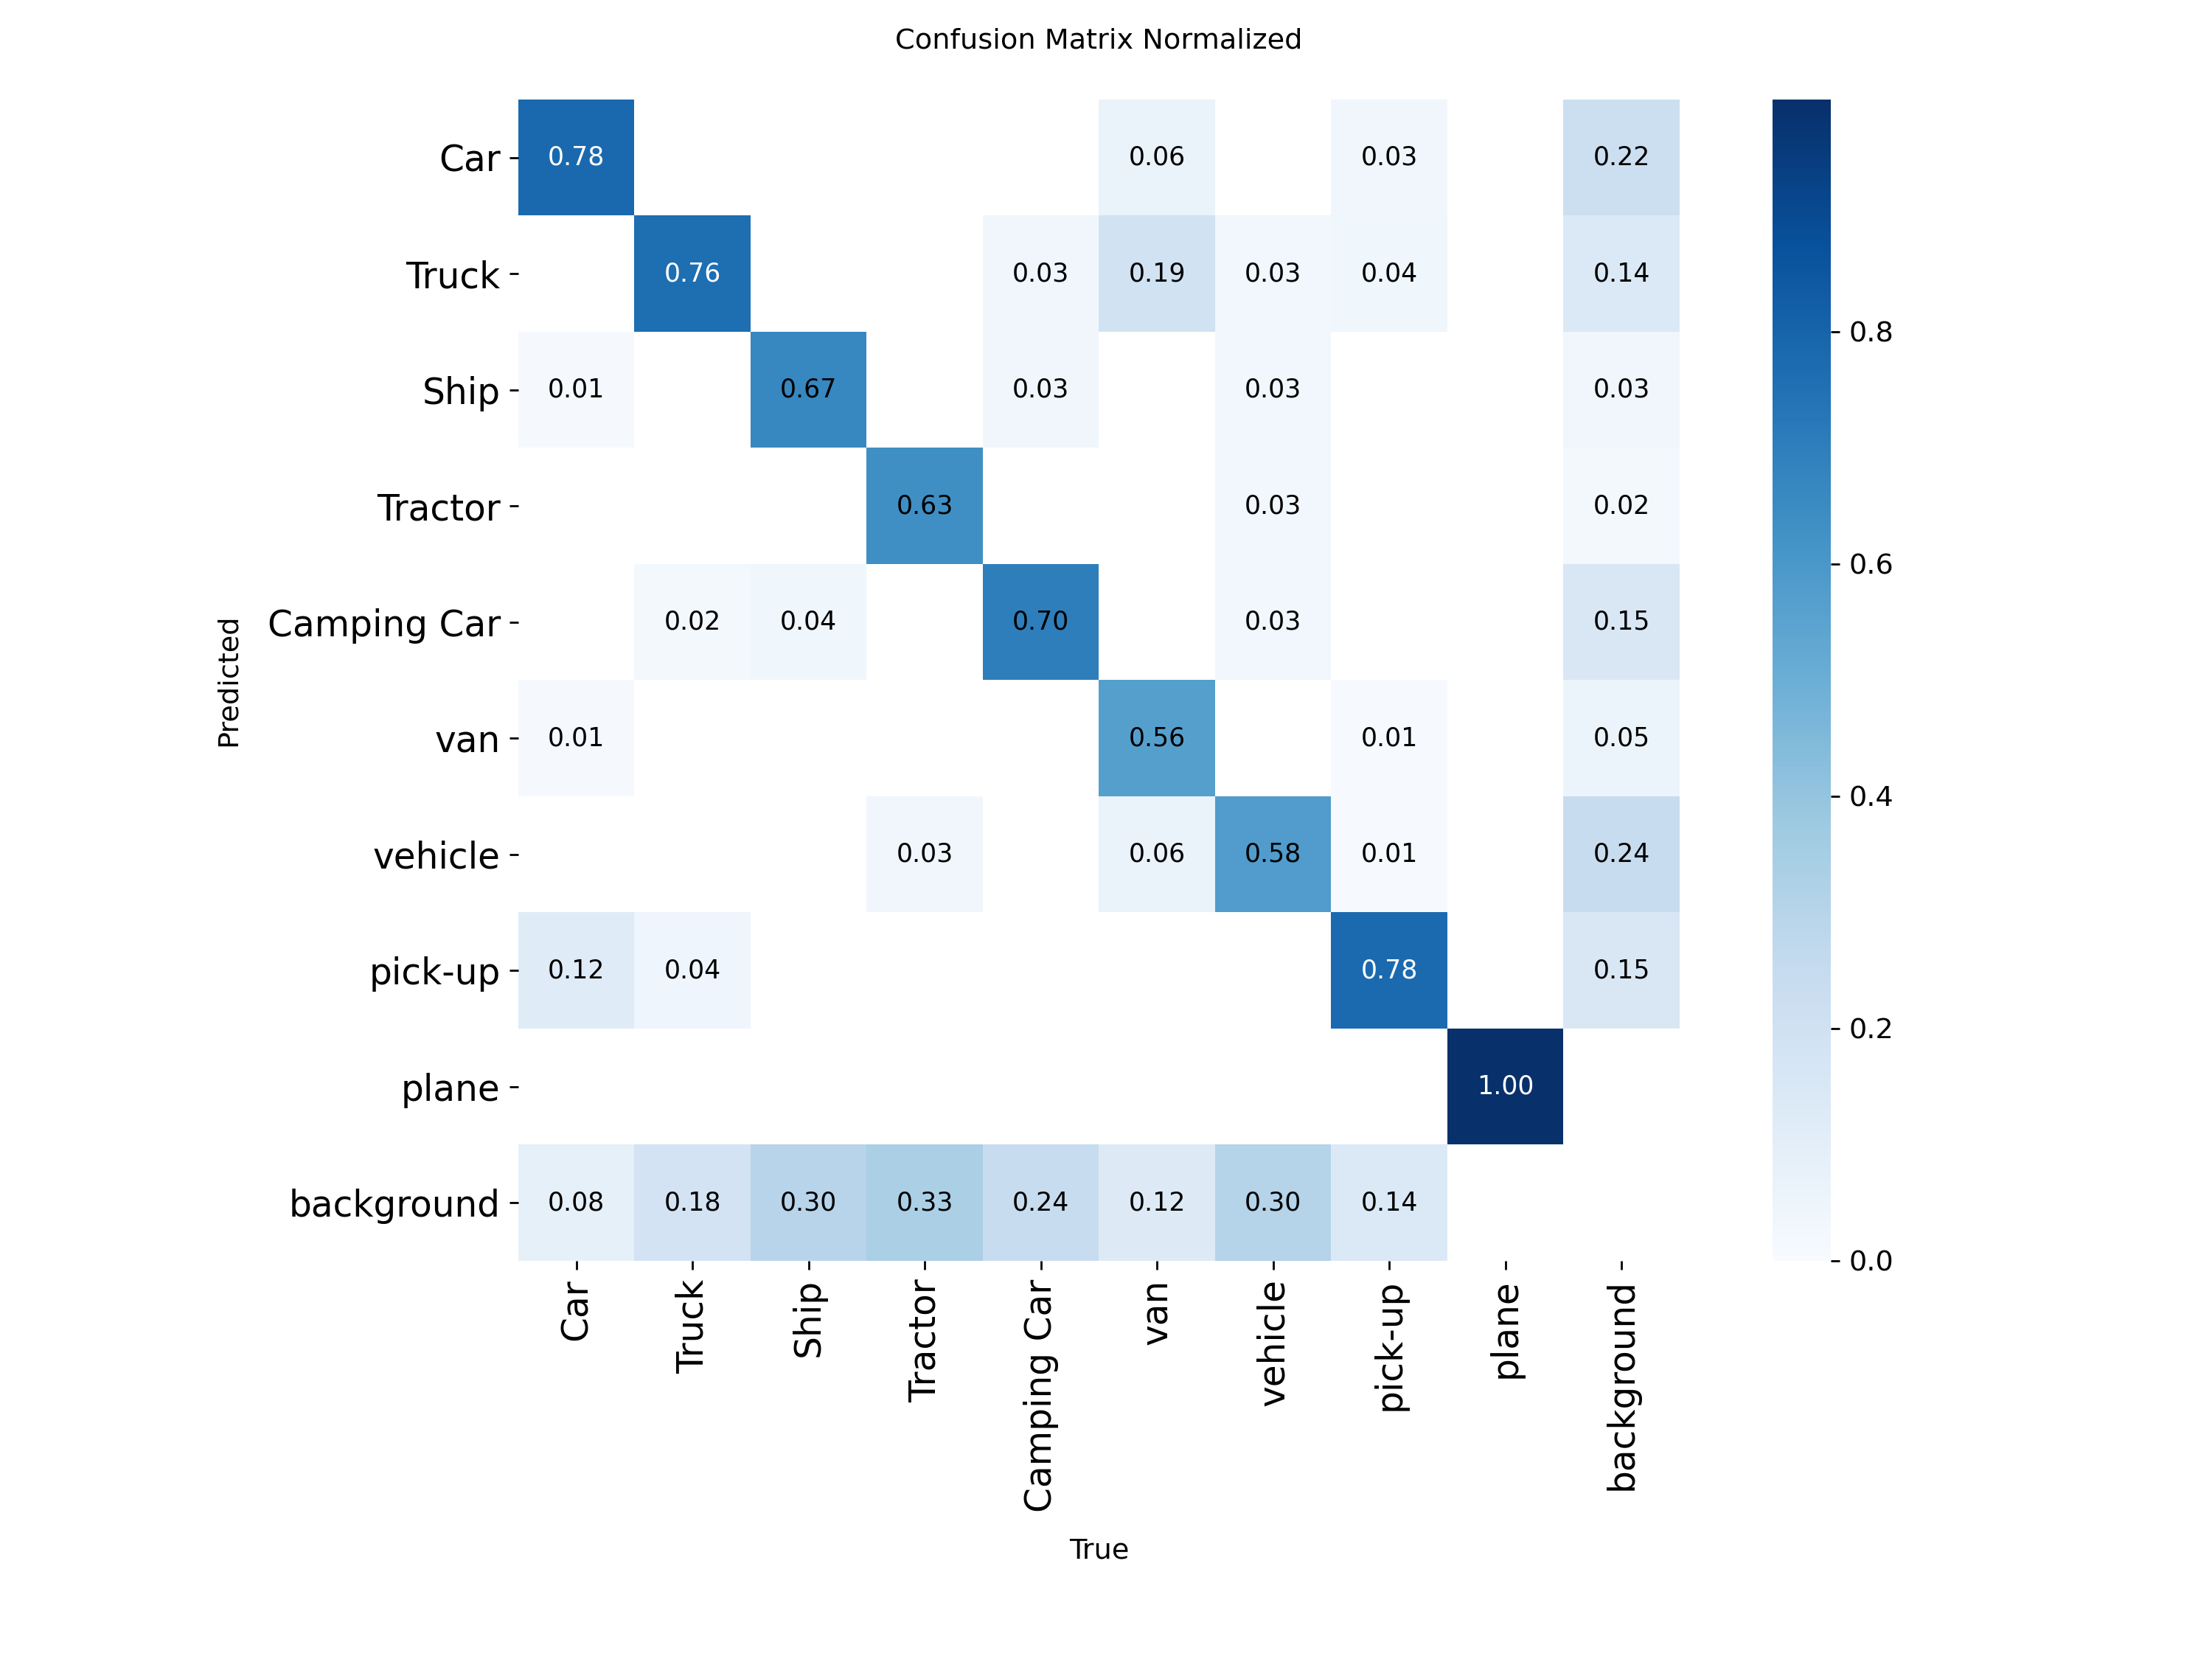
\includegraphics[width=\textwidth]{images/confusion_matrices/rgbir_F4_confusion_matrix_normalized.png} % Bildpfad zum ersten Bild
        \caption{r-g-b-ir} % Unterschrift für das erste Bild
        \label{fig:cm_trgbir} % Label für Referenzierung von Bild 1
    \end{subfigure}
    \hfill % Fügt horizontalen Platz zwischen den Subfiguren ein
    % Zweite Subfigur
    \begin{subfigure}[b]{0.85\textwidth} % 0.48\textwidth für das zweite Bild
        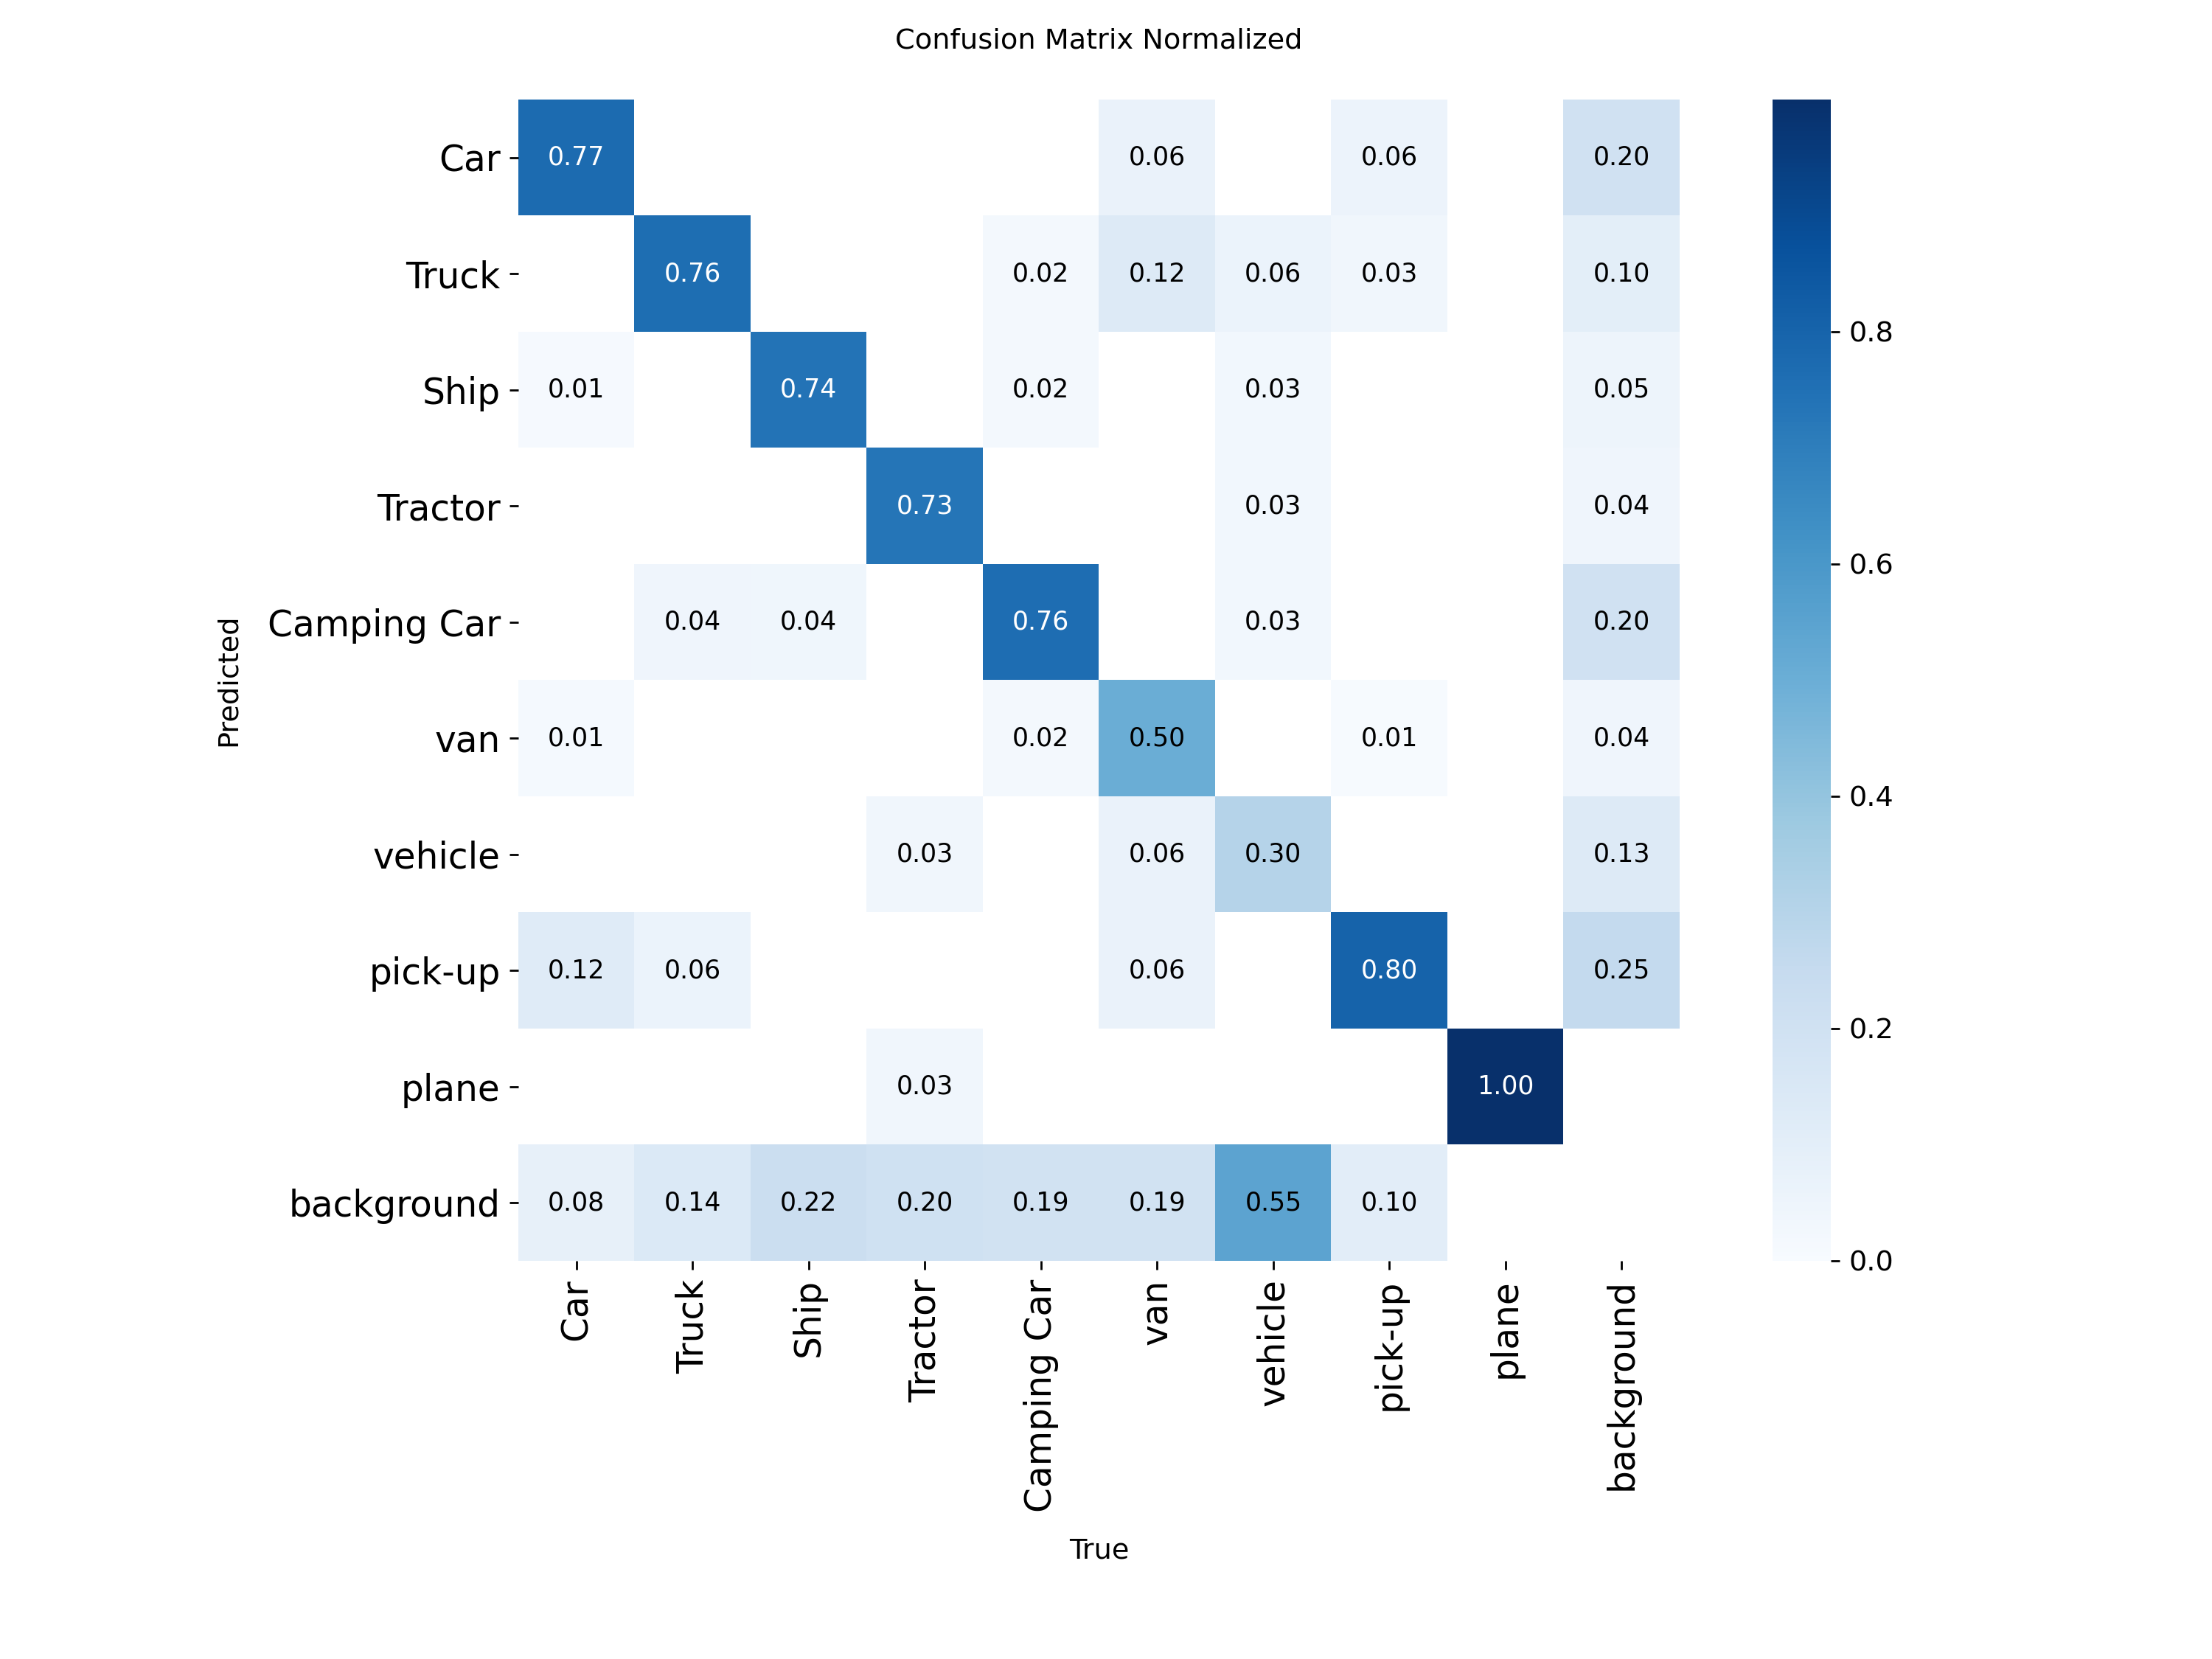
\includegraphics[width=\textwidth]{images/confusion_matrices/irgb_F4_confusion_matrix_normalized.png} % Bildpfad zum zweiten Bild
        \caption{ir-g-b} % Unterschrift für das zweite Bild
        \label{fig:cm_irgb} % Label für Referenzierung von Bild 2
    \end{subfigure}
    \caption{Comparison of Confusion Matrices between r-g-b-ir und ir-g-b for Fold 4} % Gemeinsame Unterschrift für beide Bilder
    \label{fig:combined_maps} % Label für die gesamte Figure-Umgebung
\end{figure}